\documentclass{article}
\usepackage{amsmath}
\usepackage[margin=1in]{geometry}
\usepackage{graphicx}
\usepackage{nopageno}

\setlength{\parindent}{0pt}
\setlength{\parskip}{2ex plus 1ex minus 0.5ex}

\renewcommand{\arraystretch}{1.5}

\begin{document}
\begin{center}
{\large Chestnut Oak climate reconstruction}\\
{March 2012}
\end{center}

\section{Data}




PCA percent variation explained by first three components: $0.43515425, 0.24049312, 0.17693894$.

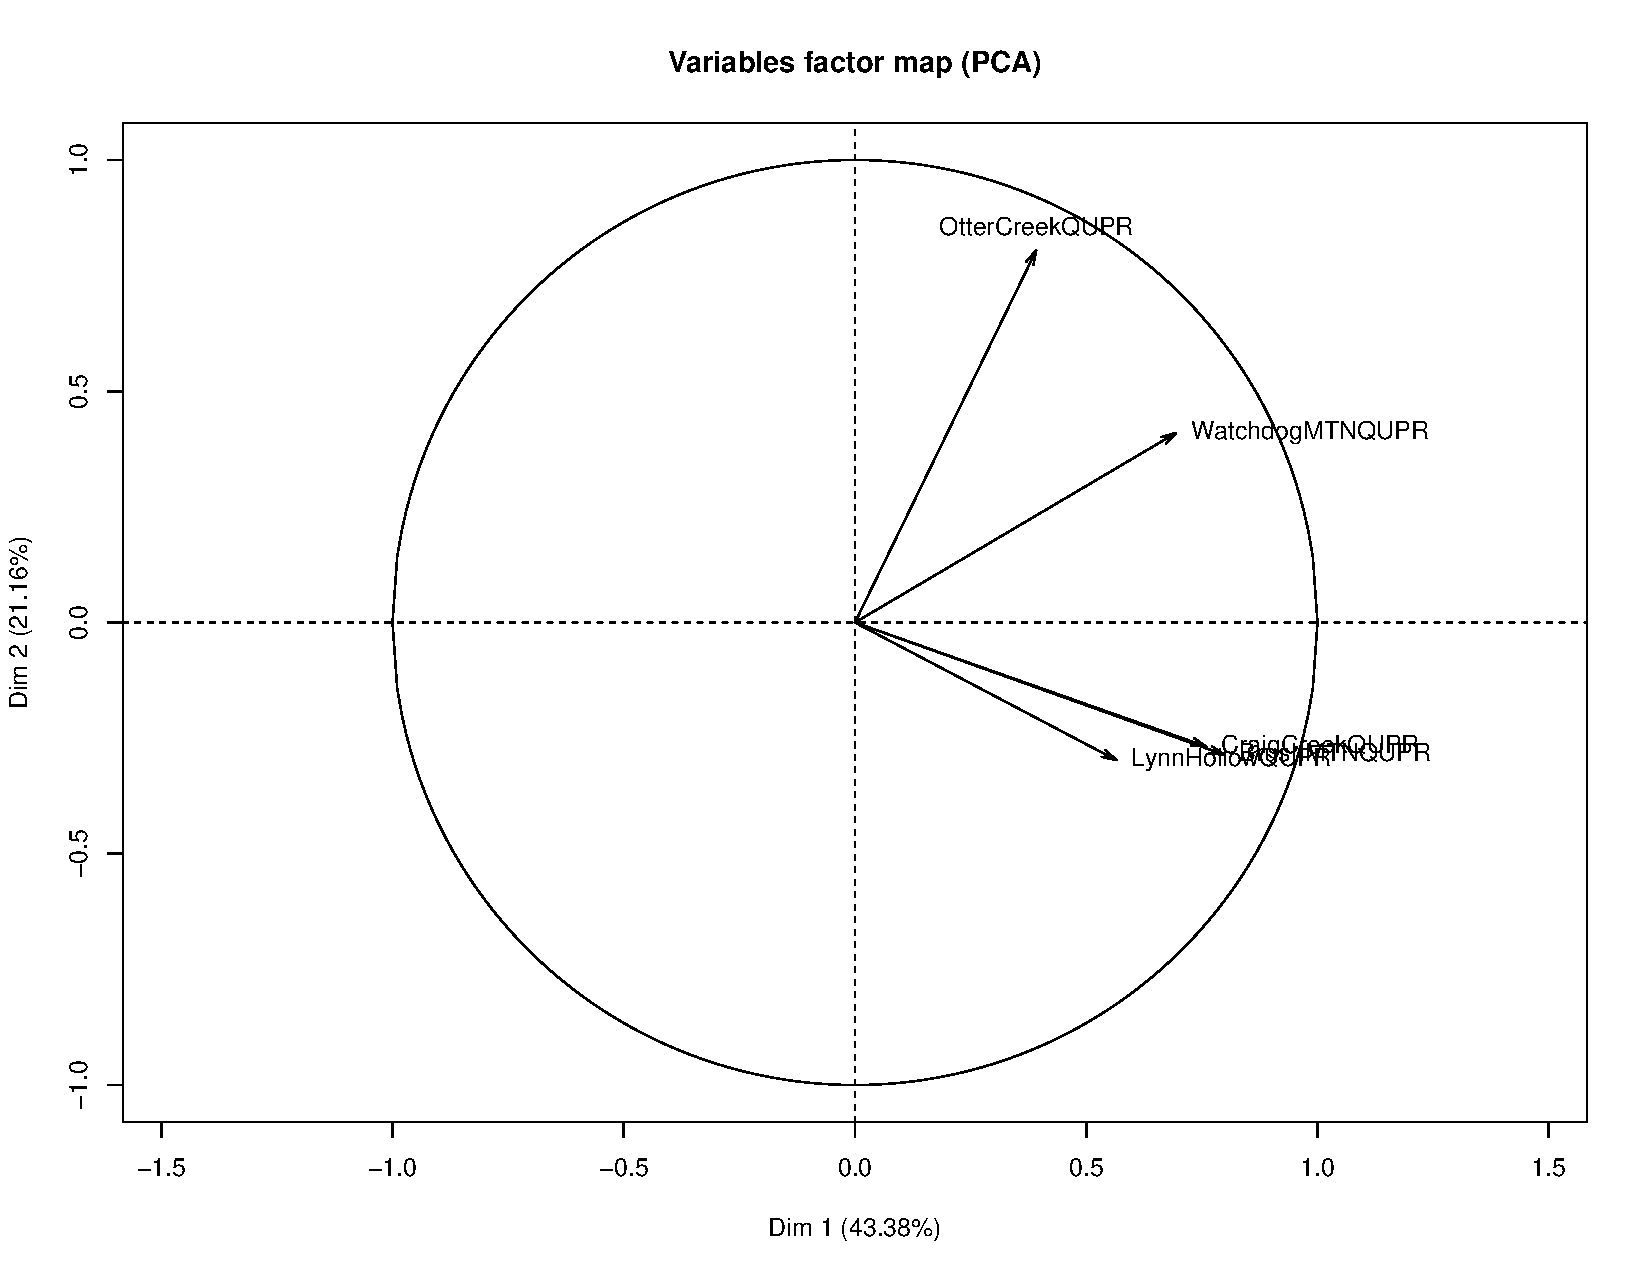
\includegraphics[width=7in]{factorMap.pdf}


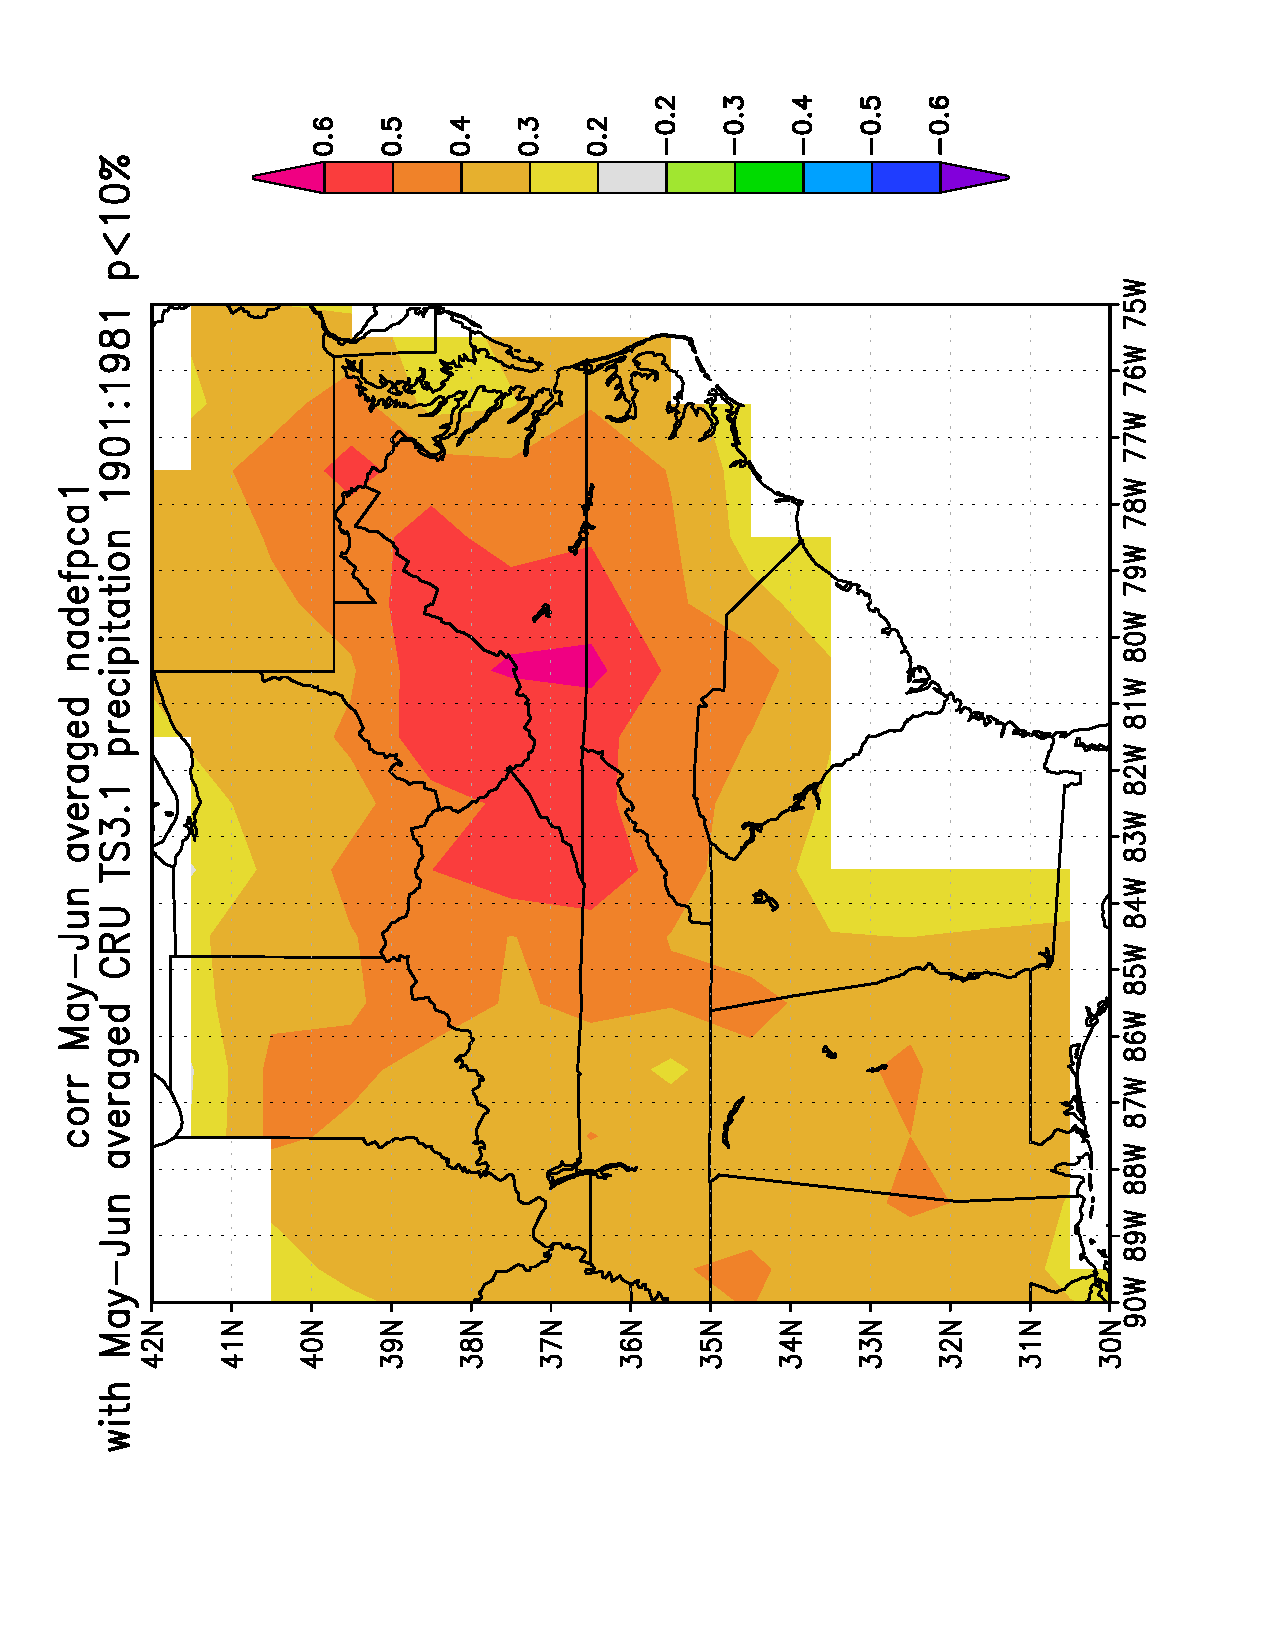
\includegraphics[width=5in, angle=-90]{MJPrecipmap.pdf}

\begin{align*}
	MSE(\hat{y}) = \sum_{i=1}^{N} (y_i - \hat{y_i})^2
\end{align*}

\begin{align*}
RE = 1 - \frac{MSE(\hat{y})}{\sum_{i=1}^{N} (y_i - \bar{y}_c)^2}
\end{align*}
\begin{align*}
CE = 1 - \frac{MSE(\hat{y})}{\sum_{i=1}^{N} (y_i - \bar{y}_v)^2},
\end{align*}
where\\
\begin{center}
\begin{tabular}{ll}
$N$ & number of years in the verification period; \\
$y_i$ & measured precip in year $i$; \\
$\bar{y}$ & mean of measured precip over calibration or verification years (indicated by subscript);\\
$\hat{y}_i$ & estimated precip in year $i$; \\
\end{tabular}
\end{center}



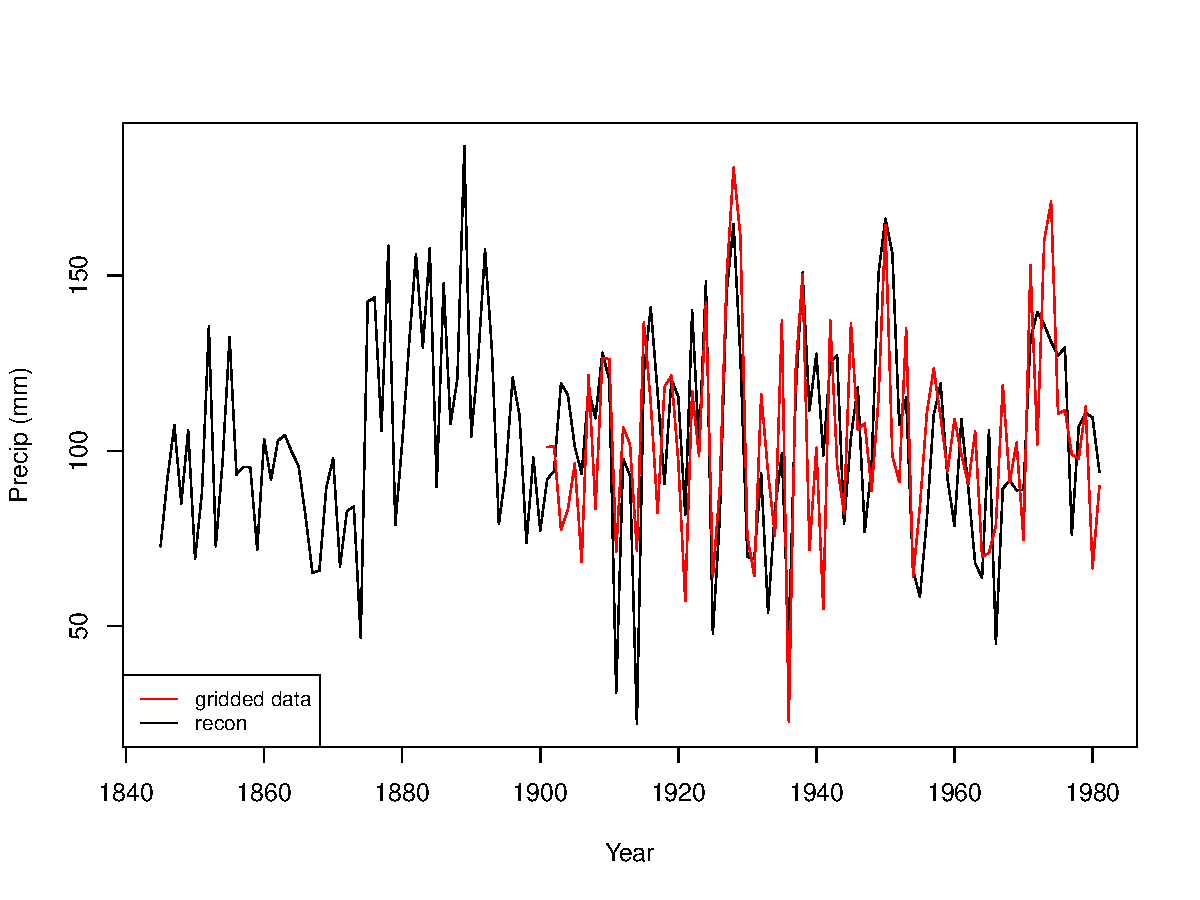
\includegraphics[width=7in]{precipRecon.pdf}




\end{document} 
